\section{Analisi del Problema}
\labelsec{ProblemAnalysis}
%===========================================================================

\paragraph{Assunzioni}
Prima di iniziare l'analisi del problema abbiamo ritenuto neccessario effettuare delle assuzioni riguardanti al paradigma che ci consentirebbe di effettuare un prodotto di qualit\'a migliore e con meno sforzi.

Il paradigma di programmazione di riferimento \'e il \textit{reactive programming} perch\'e la concezione di flusso di dati \'e proprio quello che ci interessa modellare in quanto anche nel nostro sistema sar\'a presente un flusso di dati dal client al server. Per la comunicazione attraverso la rete questo ci consente di sfruttare chiamate asincrore aumentando il disaccoppiamento tra client e server.

Per questo abbiamo deciso di utilizzare per i dati un database NoSQL per via dell'estremo dinamismo, in quanto ci consente di aggiungere dei campi anche in seguito e miglioramento di performance nell'accesso a dati che normalmente richiederebbero dei join.

Per ulteriori informazioni pi\'u dettagliate sul paradigma si rimanda ad un'altra sede. 

\subsection{Architettura Logica}

Per la costruzione dell'architettura logica ci si baser\'a ovviamente sulla precedente analisi dei requisiti in modo da mantenere il contatto con questi e non rischiare di uscire fuori specifica. Anche in questo caso si andr\'a separare l'analisi in due parti:

\begin{itemize}
\item Sistema Embedded
\item Server e Website
\end{itemize}

La parte del website \'e stata incorpata direttamente nella parte server proprio per la sua assenza di business logic.

\paragraph{Modellazione Reactive}

Prima di iniziare a costruire la modellazione sulla base del paradigma appena citato \'e necessario capire come fare a modellare lo stream stesso all'interno della nostra architettura logica, conseguentemente si \'e deciso di utilizzare i \textit{marable diagrams}. Questi sono una rappresentazione di come il flusso di dati nel tempo avviene e quali tipologie di trasformazioni consentono di effettuare.

Con questi schemi ci viene concesso ancora una volta di concentrarci prima sul ''cosa'' e non sul ''come'' che invece viene delegata alla parte progettuale, dove si cercher\'a effettivamnete di implementare il risultato finale dell'analisi

\subsubsection{Sistema Embedded}

Alla luce del paradigma di programmazione che si \'e deciso di adottare sono stati effettuati dei cambiamenti anche alla struttura che \'e stata esposta precedentemente proprio perch\'e ci sono state fornite da questa assunzione nuovi livelli di astrazione, primo tra tutti il concetto di \textbf{Stream/Flusso}. Quindi in questa fase abbiamo ritenuto molto utile iniziare a visualizzare effettivamente questi flussi tramite un'apposito diagramma.

% Figura fatta con draw.io
\begin{figure}[ht]
\centering
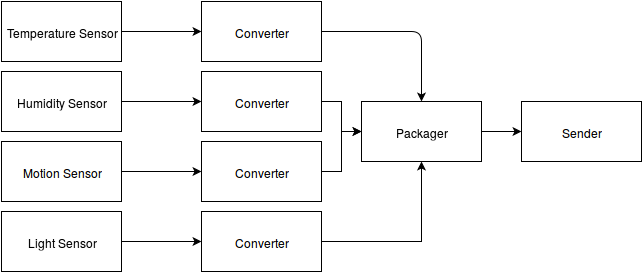
\includegraphics[width=\textwidth]{Figures/LogicArchitecture/EmbeddedSystem/FlowDiagram.png}
\caption{Diagramma di flusso, per sensore, dei dati}
\end{figure}


In particolare si puo' notare come in questo diagramma il compito di convertire i valori di un sensore sia stato disaccoppiato dal sensore stesso che quindi si deve solamente occupare di invitare i dati all'interno del flusso. \'E stato inoltre aggiunto anche una nuova entit\'a \textit{packager} che si occuper\'a di formattare i valori secondo il protocollo che deve essere definito tra client e server per l'apposita comunicazione. In particolare ogni dato proveniente da un sensore avr\'a un suo formato per via: della differenziazione dei dati, della tempistica di rilevazione che pu\'o anche risultare diversa e dell'idea percui la comunicazione in ogni caso debba essere asincrona.

Sulla base di questa ultima frase si vuole sottolineare che ogni sensore quindi avr\'a un suo flusso asincrono, ma che in quest'immagine si \'e deciso di condensare in un'unica immagine per comodit\'a.

Di seguito si indica un primo marable diagram che mostra le varie trasformazioni che verranno applicate. Questo serve soprattutto per iniziare a capire poi come interpretare eventuali altri schemi come questo.

% Figura fatta con draw.io
\begin{figure}[ht]
\centering
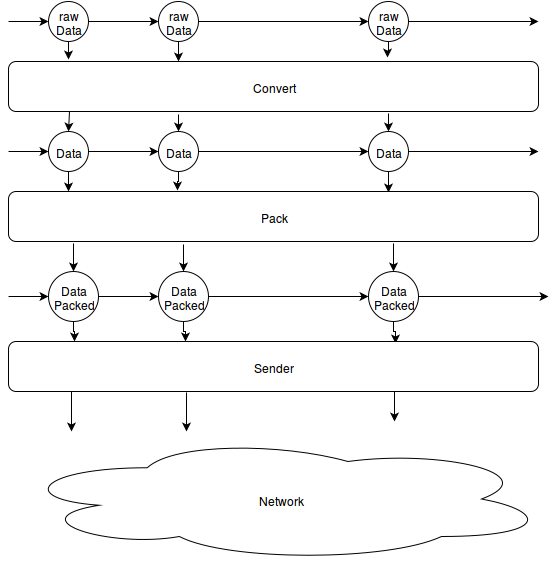
\includegraphics[scale=0.7]{Figures/LogicArchitecture/EmbeddedSystem/MarableDiagram.png}
\caption{Marable diagram dei singoli dati proveniente da una sorgente}
\end{figure}


\afterpage{\clearpage}

\newpage


\paragraph{Struttura} Chiaramente la struttura, che si basa sul precedente step di analisi dei requisiti, risulta cambiata anche alla luce delle assunzioni effettuate e quindi si possono notare l'introduzione di alcune entit\'a che servono per la gestione del sistema embedded e per impostare i flussi di dati provenienti dai sensori

\paragraph{Interazione} La parte di interazione viene drasticamente modificata proprio perch\'e l'assunzione del paradigma reactive risulta principalmente improntato su questo, in particolare \'e possibile condensare in meno codice, e pi\'u dichiarativo. Vengono in ogni caso mostrati le varie operazioni effettuate sullo stream per mantenere il contatto con quanto mostrato attraverso i marable diagrams. Particolare attenzione va posta poi sulla parte che converte da \textit{procedure calls} a \textit{reactive streams}.

\paragraph{Comportamento}

\subsection{Gap di Astrazione}

In questa sezione aggiungeremo tutti i tipi di astrazioni che sono richieste per affrontare il progetto e che non sono direttamente fruibili attraverso la tecnologia di riferimento.

\begin{enumerate}
  \item Web Server: Vista la necessit\'a di comunicare attraverso la rete \'e necessario che si utilizzi un paradigma a message-passing o attraverso chiamate asincrone, soprattutto per la comunicazione che avviene tra il raspberry e il server.
  \item Continuous Integration, Testing and collaborative source control: Lavorando in gruppo sullo stesso repository \'e necessario impostare il lavoro affinch\'e sia possibile effettuare le modifiche in maniera indipendente gli uni dagli altri e allo stesso modo sia possibile controllare automaticamente che i test predisposti e le modifiche effettuate siano coerenti con le specifiche e che il building del progetto sia in ogni caso garantito.
  \item{Paradigmi Eterogenei}: si \'e deciso di utilizzare dei paradigmi diversi dal OOP classico e questo pu\'o portare a problematiche di utilizzo, per via dell'inesperienza.Tutto questo pu\'o causare dei ritardi durante la realizzazione.
\end{enumerate}

\subsection{Analisi dei Rischi}

In questa sezione vanno elencati invece i rischi che si possono intraprendere in un progetto di questo tipo e quindi formalizzarli fin da subito, prima di eseguire l'effettiva realizzazione dello stesso in modo da poterli affontare e discutere preventivamente per essere pronti se questi si verificano.

\begin{itemize}
  \item Aumento dei Costi: \'e necessario porre particolare attenzione alla struttura hardware del sistema e di come i singoli componenti vanno ad interconnettersi assieme per evitare che si debbano affrontare dei costi aggiuntivi, una volta che il progetto \'e gi\'a avviato, causati da una qualche mancanza o per via di un'estensione del progetto in corso d'opera.
  \item Quantitativo della memoria: l'adozione di un database NoSQL porta con se un certo livello di ridondanza e quindi questo pu\'o portare ad un aumento di utilizzo della memoria e di spazio. Il tutto va valutato accuratamente durante il progetto, magari attraverso una serie di prove in base a come \'e stutturato il dato inizialmente. Se il rischio quindi \'e reale e quanto \'e critico.
  \item Integrazione tra le tecnologie: un possibile rischio riguarda la difficolt\'a nell'integrare tutte le tecnologie che devono essere sfruttate nel progetto per riuscire a colmare l'abstraction gap e quindi riuscire a completare il progetto attraverso l'analisi appena completata.
\end{itemize}
